\documentclass[a4paper]{report}
\usepackage[portuguese]{babel}
\usepackage{a4wide}
\usepackage[utf8x]

\usepackage{graphicx} % Required for inserting images
\usepackage{hyperref}
\usepackage{listings}
\usepackage{indentfirst}
\usepackage{color}
\usepackage{float}
\usepackage{xcolor}

\setlength{\parskip}{1em}

\definecolor{mygreen}{rgb}{0,0.6,0}
\definecolor{mygray}{rgb}{0.5,0.5,0.5}
\definecolor{mymauve}{rgb}{0.58,0,0.82}

\lstset{ %
  backgroundcolor=\color{white},   % choose the background color
  basicstyle=\footnotesize,        % size of fonts used for the code
  breaklines=true,                 % automatic line breaking only at whitespace
  captionpos=b,                    % sets the caption position to bottom
  commentstyle=\color{mygreen},    % comment style
  escapeinside={\%*}{*)},          % if you want to add LaTeX within your code
  keywordstyle=\color{blue},       % keyword style
  stringstyle=\color{mymauve},     % string literal style
}


\title{Programação Orientada aos Objetos - Relatório \\ \large{Grupo 7}}
\date{Maio 2023}
\author{Ana Beatriz Silva (a91678) \ Miguel Ângelo Freitas (a91635) \\ Paulo Jorge Freitas (100053) }
 
\begin{document}
	\begin{minipage}{0.9\linewidth}
        \centering
		
\includegraphics[width=0.4\textwidth]{ecum.jpg}\par\vspace{1cm}
		{\scshape\LARGE Universidade do Minho} \par
		\vspace{0.6cm}
		{\scshape\Large Licenciatura em Ciências da Computação} \par
		\maketitle
		\begin{figure}[H]
			
\includegraphics[width=0.32\linewidth]{ana.jpg}
			
\includegraphics[width=0.32\linewidth]{miguel.jpg}
			
\includegraphics[width=0.32\linewidth]{paulo.jpg}
		\end{figure}
	\end{minipage}
	
    \tableofcontents

    \pagebreak

    \chapter{Introdução}
    O presente relatório aborda a realização de um projeto, que foi proposto no âmbito da unidade curricular Programação Orientada aos Objetos, que consiste na criação de um sistema Marketplace Vintage, desenvolvido em Java, que permite a compra e venda de diversos artigos. Neste sistema de compra e venda de produtos, os utilizadores registados assumem o papel de vendedor e/ou de comprador. Um utilizador que pretenda vender algum artigo, é capaz registar o produto na plataforma, onde outros utilizadores, agora como compradores, são capaz de optar por encomendar esse artigo a partir da Vintage.

    \chapter{Classes}
    
    \section{ArtigoBase}
    
    Começamos por criar a classe ArtigoBase que aborda os artigos de uma forma menos detalhada, onde estão os identificadores que todos os artigos têm em comum, de forma a criar um artigo mais global onde podemos encontrar o código identificador do produto, a sua descrição, marca, preço base do mesmo. Ainda, é aqui que contem outras informações sobre o estado do uso do produto, o numero de donos anteriores, o seu desconto, a sua transportadora e se já fora vendido.
    
    \begin{lstlisting}[language=java]
    protected String codigo;
    protected String descricao;
    protected String marca;
    protected String precoBase;
    protected boolean isNovo;
    protected double avaliacaoEstado;
    protected double numDonosAnteriores;
    protected double desconto;
    protected boolean isVendido;
    protected Transportadora transportadora;
    protected String dono;
    \end{lstlisting}

    \section{Mala}
    
    A Classe Malas, possui informações sobre a sua dimensão, onde o desconto será sempre proporcionalmente inverso à sua dimensão; o material de que são constituídas e o ano que a coleção foi lançada. Ainda existem Malas que são Premium e cujo valor em vez de decrescer com a utilização (número de anos da carteira) aumenta com a mesma. Esse tipo de malas apresentarão uma valorização anual.

    \begin{lstlisting}[language=java]
    private String dimensao;
    private String material;
    private int anoColecao;
    private boolean isPremium;
    private double valorizacaoAnual;
    \end{lstlisting}

    \section{Sapatilha}
    
    As Sapatilhas possuem informações sobre o tamanho numérico, se possuem atacadores, a sua cor e a data de lançamento da coleção a que pertencem (todos os anos é lançada uma nova coleção). O Marketplace Vintage apenas permite que sapatilhas de coleções de anos anteriores possuam desconto, definido pelo vendedor, ou em sapatilhas da coleção mais recente acima do tamanho 45. Existe ainda sapatilhas versão Premium, na qual o seu design é desenvolvido por autores reconhecidos, onde existe uma valorização anual, isto é, quanto menor o ano de lançamento da sapatilha Premium, mais valor ela terá.

    \begin{lstlisting}[language=java]
    private int tamanho;
    private Boolean temAtacadores;
    private String cor;
    private Year dataLancamentoColecao;
    private boolean isPremium;
    \end{lstlisting}

    \section{TShirt}
    
     As T-Shirt, possuem um tamanho (que pode ser entre S,M,L ou XL) e um padrão (liso, riscas ou palmeiras). As T-Shirt com padrão liso nunca têm desconto. Os restantes padrões têm um desconto fixo de 50\% se forem produtos usados. As T-shirt não possuem versão Premium.
     
    \begin{lstlisting}[language=java]
    private Tamanho tamanho;
    private Padrao padrao; 
    \end{lstlisting}

    \section{Encomenda}
    
    A classe encomenda contém as informações de quais os artigos nela contida, a dimensão da embalagem, que pode ser grande, média ou pequena, o preço final após aplicados todos os cálculos, uma taxa de satisfação de serviço de 0.5€ para produtos novos, e 0.25€ para produtos usados, e ainda os custos de expedição.
    Esta  possuiu também um estado, mediante a etapa de processamento da encomenda, a sua data de criação, para quem está a ser dirigida e qual a transportadora encarregue pelo transporte.
    
    \begin{lstlisting}[language=java]
    private String codigo;
    private List<Artigo> artigos;
    private Dimensao dimensao;
    private double precoFinal;
    private double custosExpedicao;
    private double taxaSatisfacaoServico;
    private Estado estado;
    private LocalDate dataCriacao;
    private Utilizador utilizador;
    \end{lstlisting}


    \section{Transportadora}
    
    Na classe Transportadora, são apresentadas todas as propriedades que indicam o código, o nome, e os preços aplicados consoante o tamanho da encomenda, e o tipo de serviço. É ainda apresentado a sua margem de lucro, e se uma dada transportadora faz, ou não, serviços Premium. Apenas as transportadoras com serviço Premium podem fazer remessas de produtos Premium. O metodo calcularCustoExpedicao é capaz de calcular o custo da expedição mediante o tamanho da encomenda a transportar e se essa encomenda contem produtos Premium. Quanto maior for a encomenda, maior será o preço de expedição.
    
    
    \begin{lstlisting}[language=java]
    private String codigo;
    private String nome;
    private boolean isPremium;
    private double valorBasePequeno;
    private double valorBaseMedio;
    private double valorBaseGrande;
    private double margemLucro;
    private List<Artigo> artigos;
    \end{lstlisting}

    
    \section{Utilizador}

    A classe Utilizador possui os aspetos que os representam. Nesta classe, podemos encontrar o ID designado pela Vintage, o Nome, o Email, a sua Morada, o NIF, e as informações relativas às suas compras e vendas na Vintage.
    
    \begin{lstlisting}[language=java]
    private String codigo;
    private String email;
    private String nome;
    private String morada;
    private String numeroFiscal;
    private List<Artigo> artigosAVenda;
    private List<Artigo> artigosVendidos;
    private List<Artigo> artigosAdquiridos;
    \end{lstlisting}
    
    \section{Menus}

    O Menu é a vista do programa. É aqui que são apresentados todas as opções de funcionalidades que podemos fazer no programa. Possui vários métodos, principalmente métodos para mostrar algum tipo de informação ou mensagens de erro. Mantendo a identidade da arquitetura (Model - View - Controller).
    
    \begin{lstlisting}[language=java]
    private final Scanner scanner;
    private State state = State.INICIAL;
    private UtilizadorController utilizadorController;
    private ArtigoController artigoController;
    private EncomendaController encomendaController;
    private TransportadoraController transportadoraController;
    \end{lstlisting}
    
    \subsection{Opções do Menu Principal}
    
    A Vintage inicia com este Menu, que possui as seguintes opções:
    \par      
    \textbf{ "1. Login"} - Permite o utilizador entrar na sua conta Vintage.
    \par
    \textbf{"2. Registar"} - Permite ao utilizador registar na plataforma Vintage.
    \par
    \textbf{"3. Transportadora"} - Permite acessar o subMenu "Ver Transportadoras".
    \par
    \textbf{"4. Estatísticas"} - Permite o utilizador consultar estatísticas do programa.
    \par
    \textbf{"5. Avançar o tempo"} - Permite alterar a hora/data do programa.
    \par
    \textbf{"6. Sair"} - Permite sair da Vintage.
    \par
    \textbf{"7. Gravar"} - Permite gravar o estado atual da Vintage.
    \par
    \textbf{"8. Carregar"} - Permite carregar um estado da Vintage.
    \par

    \subsection{Opções do Menu Usuário}
    Após o  \textbf{Login ou Registo do Usuário}, são lhe concebido as seguintes opões:
    
    \textbf{"1. Gerir Artigos"} - Permite acessar o SubMenu Gerir Artigos.
    \par
    \textbf{"2. Comprar Artigos"} - Permite acessar o SubMenu Comprar.
    \par
    \textbf{"3. Ver encomenda"} - Permite consultar informações da encomenda.
    \par
    \textbf{"4. Finalizar Encomenda"} - Permite finalizar encomenda e expedir-la.
    \par
    \textbf{"5. Voltar para o menu principal"} - Permite retroceder ao Menu Principal Vintage.
    \par

    \subsection{Opções do Menu Gerir Artigo}
    Ao seguir a opção 1. do Menu Usuário, o utilizador é levado para o SubMenu \textbf{Gerir Artigo}, que possui as seguintes opções:

    \textbf{"1. Adicionar"} - Permite adicionar um novo artigo. Onde poderá fornecer informações sobre o produto em questão, mediante se é Sapatilha, T-Shirt ou Mala.
    \par
    \textbf{"2. Apagar"} - Permite apagar um dado artigo.
    \par
    \textbf{"3. Listar meus artigos"} - Permite consultar a lista de artigos para venda.
    \par
    \textbf{"4. Voltar"} - Permite voltar ao Menu anterior.
    \par

    \subsection{Opções do Menu Comprar Artigo}
    Caso no Menu Usuário, fora escolhida a opção \textbf{2. Comprar Artigo}, são mostradas as seguintes opções deste SubMenu:
    \par
    \textbf{"1. Comprar Sapatilhas"} - Permite comprar Sapatilhas. Aqui serão listadas todas as Sapatilhas disponíveis para compra.
    \par
    \textbf{"2. Comprar T-Shirt"} - Permite comprar T-Shirt. Aqui serão listadas todas as T-Shirt disponíveis para compra.
    \par
    \textbf{"3. Comprar Mala"} - Permite comprar Malas. Aqui serão listadas todas as Malas disponíveis para compra.
    \par
    
    \subsection{Opções de Ver Encomenda}
    Ao selecionar esta opção no Menu de Usuário, somos levados ao Menu com as opções sobre a encomenda. São essas opções:
    \par
    \textbf{"1. Preço Total"} - Permite consultar o Preço total da encomenda.
    \par
    \textbf{"2. Ver Artigos"} - Permite consultar quais os artigos na encomenda
    \par
    \textbf{"3. Remover Artigo"} - Permite remover um dado artigo.
    \par

    \subsection{Opções do Menu Transportadora}
    Ao seguir a opção 3. Transportadora no Menu Prinicpal, o utilizador é levado para o SubMenu \textbf{Ver Transportadoras}, que possui as seguintes opções:
    \par
    \textbf{1. Criar Transportadora} - Permite registar uma nova transportadora na Vintage.
    \par
    \textbf{2. Listar Transportadoras} - Permite consultar todas as transportadoras.
    \par
    \textbf{3. Detalhes de uma Transportadora} - Permite consultar detalhes de uma dada Transportadora.
    \par
    
    \subsection{Opções do Menu Estatísticas}
    Se no Menu Principal, fora encolhida a Opção \textbf{Estatísticas}, o utilizador será levado para as seguintes opções:
    \par
    \textbf{"1. Vendedor que mais faturou"} - Permite consultar qual vendedor que mais faturou na Vintage.
    \par
    \textbf{"2. Transportadora com mais volume de faturação"} - Permite consultar qual transportadora que mais faturou na Vintage.
    \par
    \textbf{"3. Listar Encomendas de um Vendedor"} - Permite listar todos os produtos expedidos por um dado Vendedor.
    \par
    \textbf{"4. Ordenação de maiores Vendedores/Compradores"} - Permite listar o pódio de Compradores/Vendedores.
    \par
    \textbf{"5. Dinheiro Vintage"} - Permite consultar os ganhos da Vintage.
    \par
    \textbf{"6. Voltar"} - Permite voltar ao Menu anterior.
    \par

    \section{Controllers}

    \par
    Neste projeto existe apenas uma classe Controller. Esta classe, MainController contem métodos para lidar com os pedidos que o utilizador realiza. De entre as quais:

    \begin{itemize}
        \item Artigos - Possui métodos para criar,listar, procurar e remover artigos;
        \item Usuários - Possui métodos para registar, fazer login, listar e procurar usuários;
        \item Encomendas - Possui métodos para adicionar, remover, listar, finalizar e obter preço final de uma encomenda;
        \item Transportadoras - Possui métodos para adicionar, listar, procurar e obter detalhes de uma transportadora;
        \item Save - Este método é capaz de guardar o estado do programa Vintage, num ficheiro fornecido, onde cada informação sobre os Utilizadores, as encomendas, os artigos e transportadoras são guardadas.
        \item Load - Este método é capaz de carregar o estado do mercado Vintage a partir de um ficheiro que lhe fora fornecido. Este carrega o Utilizadores, as encomendas, os artigos e as transportadoras, e as informações que contem em cada uma dessas classes, para o atual programa Vintage.
    \end{itemize}
    
    \begin{lstlisting}[language=java]
    private List<Utilizador> utilizadores;
    private List<Encomenda> encomendas;
    private List<Artigo> artigos;
    private List<Transportadora> transportadoras;
    private Utilizador utilizadorAtual;
    private Encomenda encomendaAtual;

    \end{lstlisting}
    
    \par SaveMercado - Esta Classe tem como objetivo guardar o estado do mercado.
    
    \section{Exceptions}
    
    \textbf{PrazoExpiradoException} - Para garantir que o processo de devolução de uma dada encomenda acontece corretamente, foi criada uma exceção, PrazoExpiradoException, que se assegura que o prazo de 48 horas estabelecido não expirou, e que o processo de devolução possa ocorrer.

    \textbf{UtilizadorExistenteException} - Esta Excpetion tem o propósito de impedir que um utilizador se registe na Vintage com informações pessoais iguais a algum perfil já existente (NIF, email).

    \textbf{UtilizadorNaoExistenteException} - Esta Exception impede de aceder a um perfil de utilizador que não existe.
    
    \textbf{EncomendaNaoExisteException} - Esta Exception atua quando o utilizador tenta aceder a uma encomenda que não existe.

    \
    \section{VintageMarketplace}
    \par Esta classe é a classe principal, responsável por inicializar todas as componentes do programa.


    \chapter{Descrição da Aplicação}
    \par Este projeto foi desenvolvido seguindo as normas da estrutura MVC - Model View Controller, ou seja, uma forma de organizar o código em três componentes distintas e independentes, cada uma com a sua responsabilidade específica:
    \begin{itemize}
    \item \textbf{Model} - O Model é responsável por armazenar e gerir o estado do programa, tal como realizar as operações necessárias nos dados. Fazem parte do Model as classes Artigo, Utilizador, Encomenda, Sapatilhas, T-Shirt, Mala, Transportadora e Artigo-Base.
    
    \item \textbf{View} - É a camada responsável pela apresentação das informações ao utilizador. O Menu faz parte desta camada.
    
    \item \textbf{Controller} - Ele atua como intermediário entre o model e a view, recebendo as solicitações do usuário, atualizando o modelo, e, em seguida, atualizando a view para refletir as mudanças no modelo.
    A classe MainController compõe o Controller da Vintage.
    
    \end{itemize}
    
    \chapter{Diagrama de Classes}
		\begin{figure}[H]
			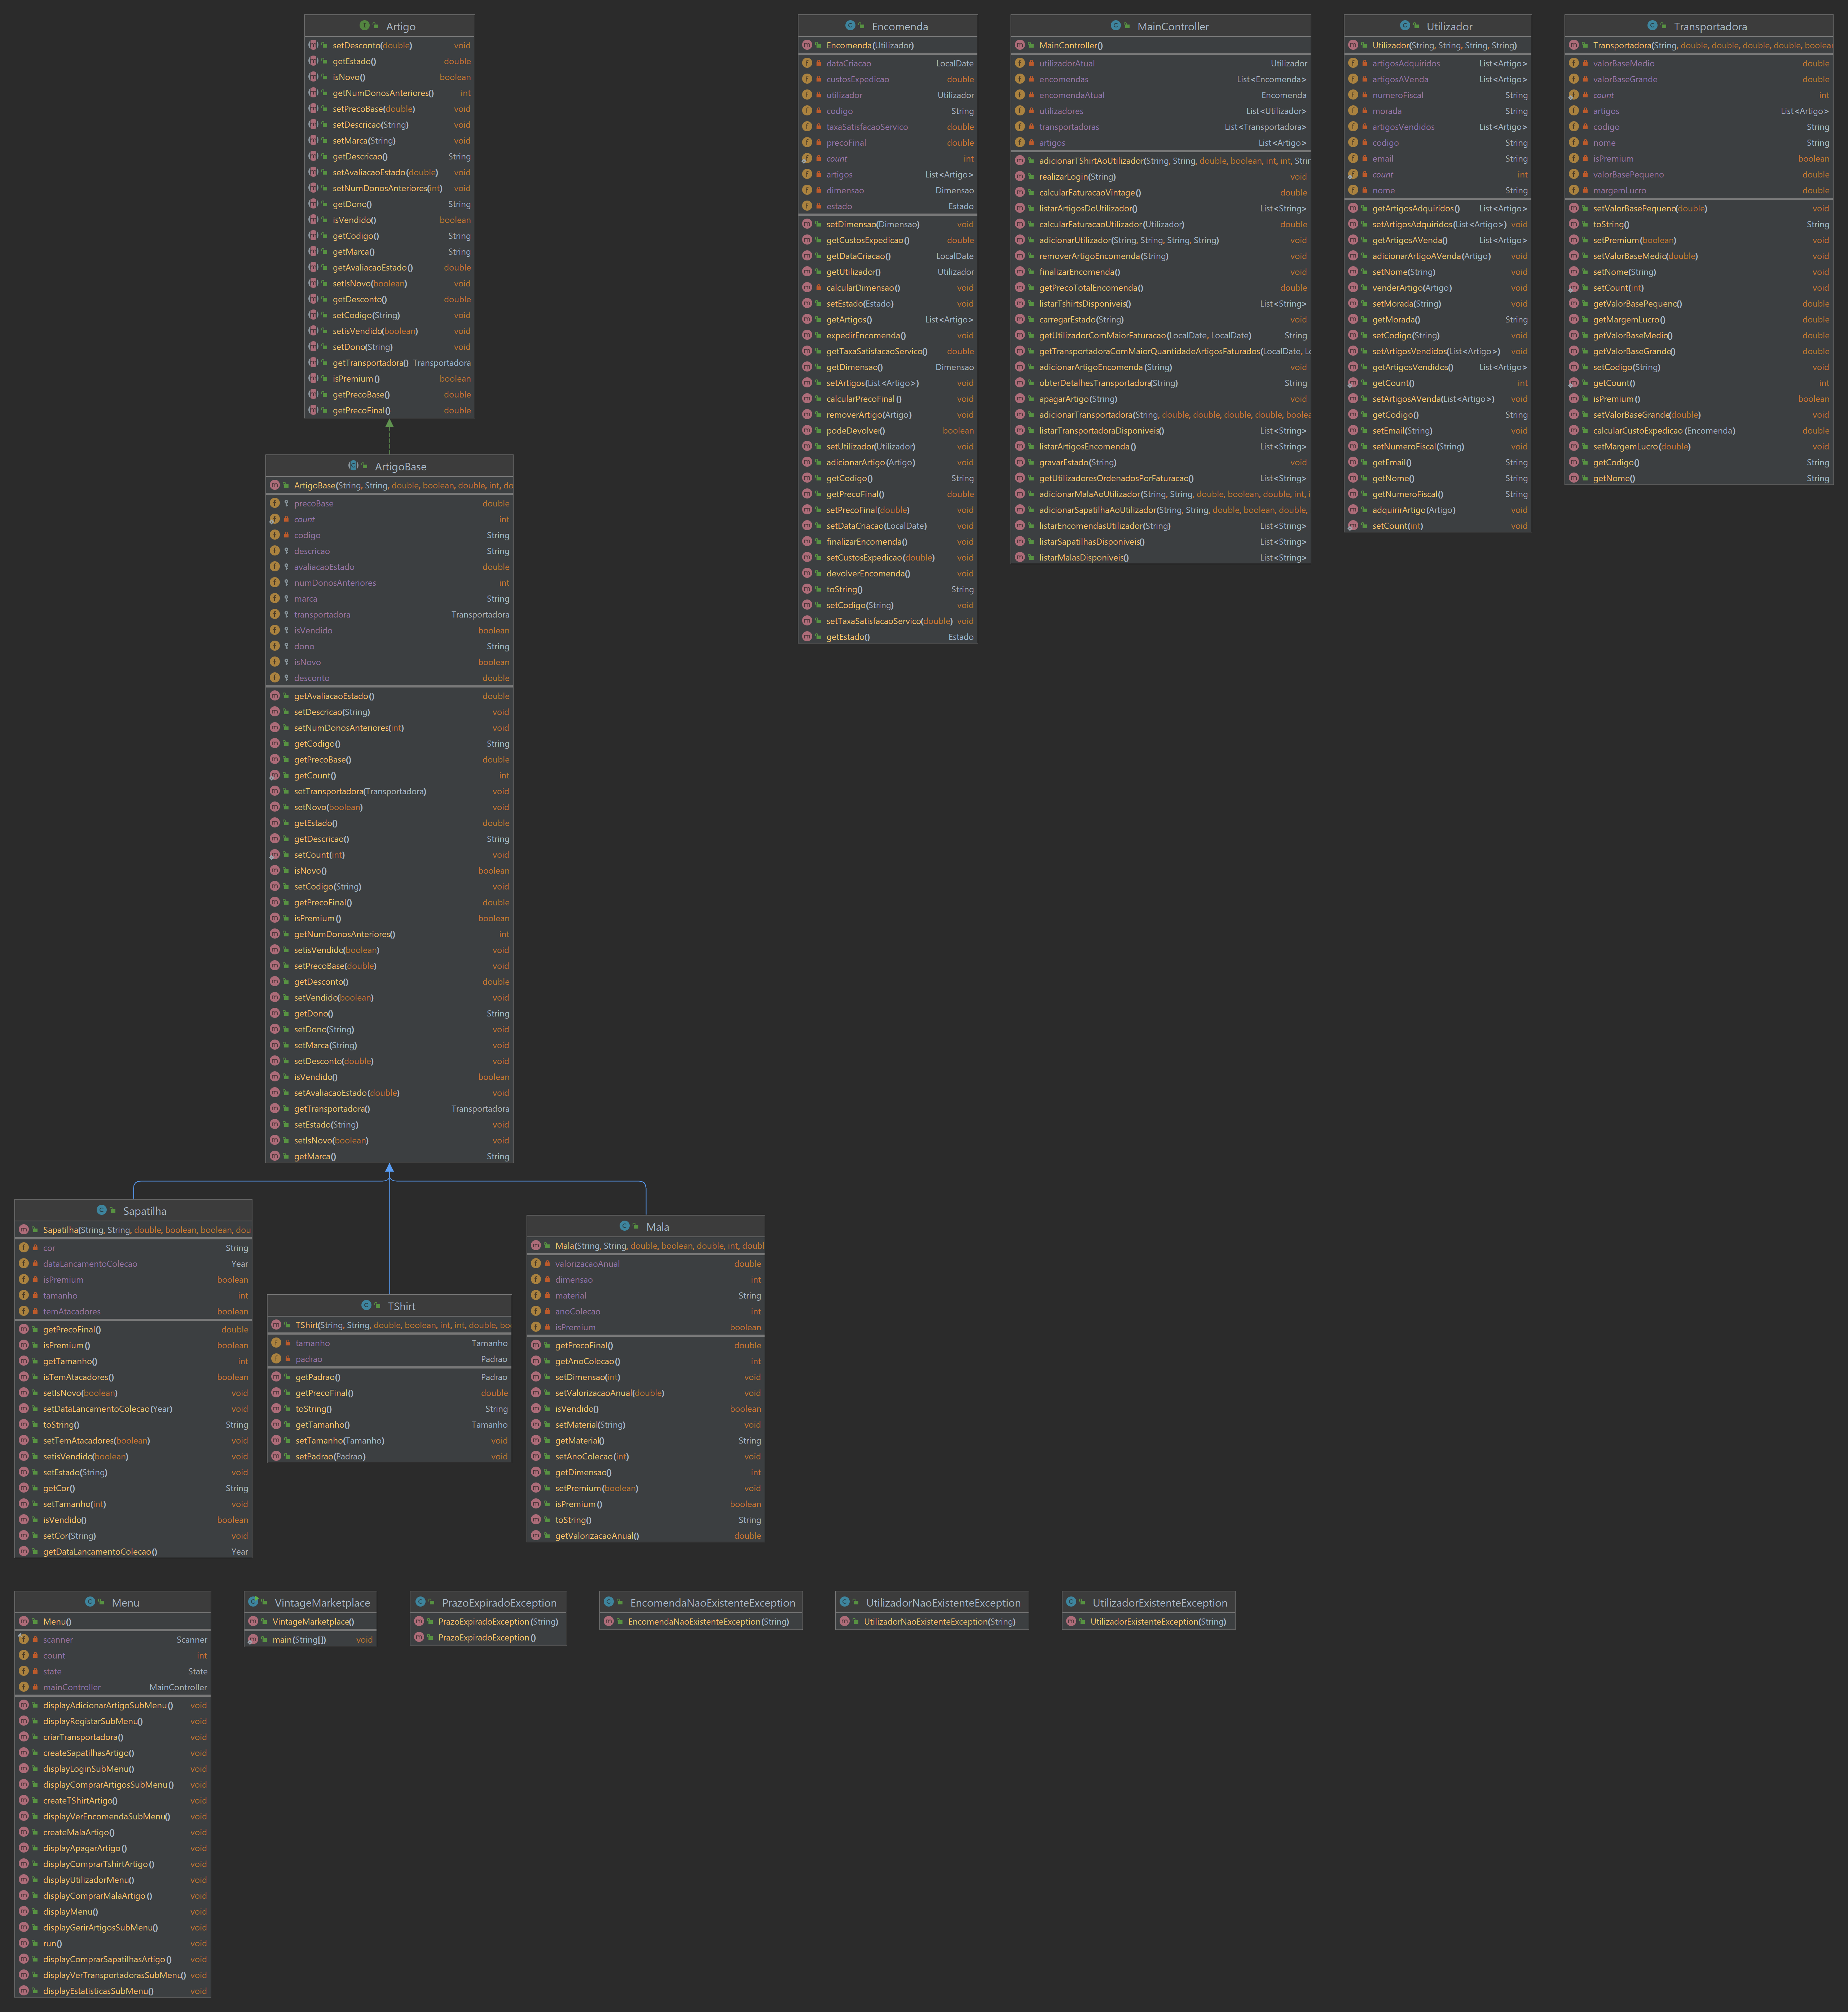
\includegraphics[scale = 0.07]{diagrama.png}
                \caption{Diagrama-Esquema do Projeto Marketplace Vintage}
		\end{figure}

    \chapter{Conclusão}
    \par Um dos principais desafios, numa fase inicial, foi a comunicação do grupo, pois nem sempre era possível reunir todos os elementos presencialmente. Com isto, foram criadas algumas barreiras à disposição de ideias e opiniões. Após uma melhor organização da nossa parte e, à medida que a nossa perceção do conteúdo da UC evoluía, fomos tomando algum rumo do trabalho, porém novas dificuldades surgiam devido a, muitas vezes, não sabermos lidar com certos problemas que apareciam ao longo da realização do trabalho.
    \par
    A nível geral, consideramos que o grupo conseguiu cumprir os objetivos propostos e, mesmo com bastantes dificuldades acreditamos que desenvolvemos uma plataforma MarketPlace Vintage tal como pedido.
    \par


\end{document}
